\documentclass[10pt,twocolumn,a4paper]{article}
\usepackage[a4paper,left=16mm,right=16mm,top=21mm,bottom=20mm,columnsep=6mm,headsep=6mm]{geometry}
\usepackage[T1]{fontenc}
\usepackage{mathptmx}
\usepackage[letterspace=180]{microtype}
\usepackage{amsmath,amssymb,amsthm,bm}
\usepackage{pifont}
\usepackage{marvosym}
\usepackage{graphicx}
\usepackage{booktabs,array,multirow}
\usepackage{colortbl}
\usepackage{placeins}
\usepackage{cite}
\usepackage{xcolor}
\definecolor{dgblue}{HTML}{1B3A5C}
\definecolor{dgrule}{HTML}{9A9A9A}
\definecolor{dgpale}{HTML}{F3F5F8}
\definecolor{dgamber}{HTML}{B8741A}
\definecolor{dgpaleamber}{HTML}{FBF4EA}
\definecolor{dghead}{HTML}{EDF0F4}
\usepackage[font={footnotesize},labelfont=bf,labelsep=space,justification=justified,singlelinecheck=false,figurename=Fig.,skip=4pt]{caption}
\captionsetup[table]{labelsep=newline,position=top}
\usepackage{titlesec}
\usepackage{needspace}
\usepackage{enumitem}
\usepackage{fancyhdr}
\usepackage[most]{tcolorbox}
\usepackage[colorlinks=true,allcolors=dgblue]{hyperref}
\usepackage{xurl}
\urlstyle{same}
% tables: blue rules, shaded header row
\arrayrulecolor{dgblue}
\setlength{\heavyrulewidth}{0.9pt}\setlength{\lightrulewidth}{0.45pt}
\setlength{\aboverulesep}{0pt}\setlength{\belowrulesep}{0pt}
\renewcommand{\arraystretch}{1.22}
% thin rule between the two columns
\setlength{\columnseprule}{0.3pt}
\usepackage{etoolbox}\makeatletter\patchcmd{\@outputdblcol}{\normalcolor\vrule}{\color{dgblue!25}\vrule}{}{}\makeatother
% key-results box
\newtcolorbox{keyresults}[1][]{enhanced,breakable,colback=white,colframe=dgblue,boxrule=0.6pt,arc=1.5pt,
  left=6pt,right=6pt,top=4pt,bottom=4pt,fontupper=\small,before skip=8pt,after skip=8pt,
  title={\small\bfseries Principal findings#1},coltitle=white,colbacktitle=dgblue,toptitle=1pt,bottomtitle=1pt}
\newcommand{\NumBaseGapMin}{0.27}
\newcommand{\NumBaseGapMax}{0.40}
\newcommand{\NumBaseGainMin}{0.00}
\newcommand{\NumBaseGainMax}{0.02}
\newcommand{\NumBaseSensMin}{0.00}
\newcommand{\NumBaseSensMax}{0.02}
\newcommand{\NumBaseSampMin}{-0.01}
\newcommand{\NumBaseSampMax}{0.00}
\newcommand{\NumBaseGainSig}{10}
\newcommand{\NumBaseSampNull}{11}
\newcommand{\NumBaseHzA}{83}
\newcommand{\NumBaseHzB}{113}
\newcommand{\NumBaseFiveSig}{12}
\newcommand{\NumBaseMaxSig}{12}
\newcommand{\NumBaseEceMMin}{0.03}
\newcommand{\NumBaseEceMMax}{0.07}
\newcommand{\NumBaseEceOMin}{0.04}
\newcommand{\NumBaseEceOMax}{0.13}
\newcommand{\NumBaseEcePMin}{0.34}
\newcommand{\NumBaseEcePMax}{0.43}
\newcommand{\NumLagGapMin}{0.27}
\newcommand{\NumLagGapMax}{0.40}
\newcommand{\NumLagGainMin}{0.01}
\newcommand{\NumLagGainMax}{0.04}
\newcommand{\NumLagSensMin}{0.00}
\newcommand{\NumLagSensMax}{0.01}
\newcommand{\NumLagSampMin}{-0.01}
\newcommand{\NumLagSampMax}{0.00}
\newcommand{\NumLagGainSig}{12}
\newcommand{\NumLagSampNull}{11}
\newcommand{\NumLagHzA}{83}
\newcommand{\NumLagHzB}{113}
\newcommand{\NumLagFiveSig}{11}
\newcommand{\NumLagMaxSig}{12}
\newcommand{\NumLagEceMMin}{0.01}
\newcommand{\NumLagEceMMax}{0.07}
\newcommand{\NumLagEceOMin}{0.05}
\newcommand{\NumLagEceOMax}{0.13}
\newcommand{\NumLagEcePMin}{0.34}
\newcommand{\NumLagEcePMax}{0.44}
\newcommand{\NumLowGapMin}{0.28}
\newcommand{\NumLowGapMax}{0.40}
\newcommand{\NumLowGainMin}{0.00}
\newcommand{\NumLowGainMax}{0.02}
\newcommand{\NumLowSensMin}{0.00}
\newcommand{\NumLowSensMax}{0.02}
\newcommand{\NumLowSampMin}{-0.01}
\newcommand{\NumLowSampMax}{0.01}
\newcommand{\NumLowGainSig}{8}
\newcommand{\NumLowSampNull}{10}
\newcommand{\NumLowHzA}{120}
\newcommand{\NumLowHzB}{154}
\newcommand{\NumLowFiveSig}{11}
\newcommand{\NumLowMaxSig}{12}
\newcommand{\NumLowEceMMin}{0.02}
\newcommand{\NumLowEceMMax}{0.11}
\newcommand{\NumLowEceOMin}{0.02}
\newcommand{\NumLowEceOMax}{0.14}
\newcommand{\NumLowEcePMin}{0.34}
\newcommand{\NumLowEcePMax}{0.44}
\newcommand{\NumCombGapMin}{0.28}
\newcommand{\NumCombGapMax}{0.40}
\newcommand{\NumCombGainMin}{0.00}
\newcommand{\NumCombGainMax}{0.02}
\newcommand{\NumCombSensMin}{0.00}
\newcommand{\NumCombSensMax}{0.01}
\newcommand{\NumCombSampMin}{-0.01}
\newcommand{\NumCombSampMax}{0.01}
\newcommand{\NumCombGainSig}{10}
\newcommand{\NumCombSampNull}{12}
\newcommand{\NumCombHzA}{201}
\newcommand{\NumCombHzB}{258}
\newcommand{\NumCombFiveSig}{11}
\newcommand{\NumCombMaxSig}{12}
\newcommand{\NumCombEceMMin}{0.02}
\newcommand{\NumCombEceMMax}{0.09}
\newcommand{\NumCombEceOMin}{0.02}
\newcommand{\NumCombEceOMax}{0.13}
\newcommand{\NumCombEcePMin}{0.34}
\newcommand{\NumCombEcePMax}{0.43}
\newcommand{\NumLisGapMin}{0.09}
\newcommand{\NumLisGapMax}{0.34}
\newcommand{\NumLisGainMin}{0.00}
\newcommand{\NumLisGainMax}{0.02}
\newcommand{\NumLisSensMin}{0.01}
\newcommand{\NumLisSensMax}{0.02}
\newcommand{\NumLisSampMin}{-0.01}
\newcommand{\NumLisSampMax}{0.01}
\newcommand{\NumLisGainSig}{8}
\newcommand{\NumLisSampNull}{12}
\newcommand{\NumLisHzA}{100}
\newcommand{\NumLisHzB}{202}
\newcommand{\NumLisFiveSig}{12}
\newcommand{\NumLisMaxSig}{12}
\newcommand{\NumLisEceMMin}{0.08}
\newcommand{\NumLisEceMMax}{0.41}
\newcommand{\NumLisEceOMin}{0.11}
\newcommand{\NumLisEceOMax}{0.44}
\newcommand{\NumLisEcePMin}{0.34}
\newcommand{\NumLisEcePMax}{0.45}
\newcommand{\NumLinConst}{90}
\newcommand{\NumLinExc}{53}
\newcommand{\NumLinErr}{-4}
\newcommand{\NumLinErrAbs}{4}
\newcommand{\NumCbN}{51}
\newcommand{\NumCbB}{0.0256}
\newcommand{\NumCbT}{-6.6}
\newcommand{\NumCbSd}{0.16}
\newcommand{\NumCbBias}{1.62}
\newcommand{\NumLisN}{46}
\newcommand{\NumLisHeld}{53}
\newcommand{\NumLisB}{0.0235}
\newcommand{\NumLisT}{-2.3}
\newcommand{\NumLisBLo}{0.0203}
\newcommand{\NumLisBHi}{0.0265}
\newcommand{\NumLisTLo}{-4.2}
\newcommand{\NumLisTHi}{-0.9}
\newcommand{\NumLisBiasHeld}{1.02}
\newcommand{\NumLisAccHeld}{1.37}
\newcommand{\NumLisAccFit}{1.33}
\newcommand{\NumLisGen}{32}
\newcommand{\NumLisRatio}{5.9}
\newcommand{\NumLisSd}{0.38}
\newcommand{\NumLisOrcAMin}{0.88}
\newcommand{\NumLisOrcAMax}{0.92}
\newcommand{\NumLisOrcBMin}{1.00}
\newcommand{\NumLisOrcBMax}{1.00}
\newcommand{\NumLisEceAMMin}{0.28}
\newcommand{\NumLisEceAMMax}{0.41}
\newcommand{\NumLisEceAPMin}{0.42}
\newcommand{\NumLisEceAPMax}{0.45}
\newcommand{\NumLisEceBMMin}{0.08}
\newcommand{\NumLisEceBMMax}{0.20}
\newcommand{\NumLisEceBPMin}{0.34}
\newcommand{\NumLisEceBPMax}{0.41}
\newcommand{\NumLisPrevMin}{0.08}
\newcommand{\NumLisPrevMax}{0.38}

\newcommand{\DatNFull}{373}
\newcommand{\DatNLis}{102}
\newcommand{\DatNSp}{51}
\newcommand{\TabAUC}{\begin{table*}[t]\centering\footnotesize
\caption{AUC of the five scores from a DS18B20 record sampled every 15\,min (baseline run, 4\,000 trips per row). The best score in each row is in bold. The last two columns give the same kinetic score with an ideal sensor sampled every minute, and the oracle that knows each trip's biology}\label{tab:auc}
\begin{tabular}{@{}lllccccccc@{}}\toprule\rowcolor{dghead}
Limit & Product & $cv$ & CSL & Degree-h $>4$\,\textdegree C & Time $>5$\,\textdegree C & Time $>8$\,\textdegree C & $T_{\max}$ & Ideal, 1 min & Oracle\\\midrule
A & Pouch & 0.00 & \textbf{0.705} & 0.690 & 0.635 & 0.569 & 0.629 & 0.718 & 1.000\\
A & Pouch & 0.10 & \textbf{0.651} & 0.634 & 0.599 & 0.557 & 0.591 & 0.659 & 1.000\\
A & Pouch & 0.25 & \textbf{0.620} & 0.619 & 0.591 & 0.561 & 0.602 & 0.627 & 1.000\\
A & Crate & 0.00 & \textbf{0.722} & 0.711 & 0.701 & 0.586 & 0.638 & 0.732 & 1.000\\
A & Crate & 0.10 & \textbf{0.674} & 0.666 & 0.657 & 0.577 & 0.611 & 0.687 & 1.000\\
A & Crate & 0.25 & \textbf{0.599} & 0.596 & 0.592 & 0.541 & 0.571 & 0.603 & 1.000\\
\midrule
B & Pouch & 0.00 & \textbf{0.710} & 0.686 & 0.636 & 0.564 & 0.587 & 0.723 & 1.000\\
B & Pouch & 0.10 & \textbf{0.656} & 0.634 & 0.606 & 0.539 & 0.564 & 0.670 & 1.000\\
B & Pouch & 0.25 & \textbf{0.604} & 0.594 & 0.565 & 0.531 & 0.549 & 0.608 & 1.000\\
B & Crate & 0.00 & \textbf{0.708} & 0.696 & 0.687 & 0.600 & 0.629 & 0.724 & 1.000\\
B & Crate & 0.10 & \textbf{0.676} & 0.670 & 0.663 & 0.585 & 0.611 & 0.686 & 1.000\\
B & Crate & 0.25 & \textbf{0.603} & 0.595 & 0.591 & 0.538 & 0.552 & 0.608 & 1.000\\
\bottomrule\end{tabular}\end{table*}}

\newcommand{\TabBudget}{\begin{table}[t]\centering\footnotesize
\caption{Loss budget: mean AUC over the 12 settings of each run as information is removed, and the range of the biology gap (oracle minus ideal sensor)}\label{tab:budget}
\setlength{\tabcolsep}{3.2pt}
\begin{tabular}{@{}lcccccc@{}}\toprule\rowcolor{dghead}
Run & Oracle & Ideal & PT1000 & DS18B20 & DS18B20 & Biology gap\\
 & & 1\,min & 15\,min & 15\,min & 60\,min & \\\midrule
Baseline & 1.000 & 0.671 & 0.670 & 0.661 & 0.662 & 0.27--0.40\\
Extra lag & 0.988 & 0.652 & 0.652 & 0.644 & 0.645 & 0.27--0.40\\
Low load & 1.000 & 0.667 & 0.666 & 0.656 & 0.657 & 0.28--0.40\\
Milk flora & 1.000 & 0.664 & 0.663 & 0.654 & 0.653 & 0.28--0.40\\
\textit{Listeria} & 0.950 & 0.738 & 0.737 & 0.725 & 0.726 & 0.09--0.34\\
\bottomrule\end{tabular}\end{table}}

\newcommand{\TabContrasts}{\begin{table*}[t]\centering\footnotesize
\caption{Paired AUC differences on identical trips: minimum/maximum over the 12 settings of each run, with the number of settings (of 12) whose 95\,\% paired-bootstrap interval excludes zero in brackets}\label{tab:contrasts}
\begin{tabular}{@{}lccccc@{}}\toprule\rowcolor{dghead}
Contrast & Baseline & Extra lag & Low load & Milk flora & \textit{Listeria}\\\midrule
CSL $-$ degree-h & 0.001/0.023 (10) & 0.006/0.037 (12) & 0.001/0.023 (8) & 0.004/0.025 (10) & 0.002/0.023 (8)\\
CSL $-$ time $>5$\,\textdegree C & 0.008/0.074 (12) & 0.001/0.104 (11) & 0.005/0.066 (11) & 0.006/0.075 (11) & 0.010/0.077 (12)\\
PT1000 $-$ DS18B20 & 0.003/0.015 (9) & 0.003/0.013 (7) & 0.005/0.018 (10) & 0.002/0.015 (8) & 0.005/0.020 (8)\\
60\,min $-$ 1\,min & -0.008/0.004 (1) & -0.008/0.004 (1) & -0.011/0.008 (2) & -0.009/0.006 (0) & -0.008/0.009 (0)\\
Adaptive $-$ 1\,min & -0.006/0.005 (0) & -0.006/0.006 (0) & -0.008/0.009 (1) & -0.007/0.006 (0) & -0.006/0.009 (0)\\
\bottomrule\end{tabular}\end{table*}}

\newcommand{\TabCal}{\begin{table*}[t]\centering\footnotesize
\caption{Calibration: range of expected calibration error over the 12 settings, and mean Brier score, for each run. Lower is better}\label{tab:cal}
\begin{tabular}{@{}lccccc@{}}\toprule\rowcolor{dghead}
Variant & Baseline & Extra lag & Low load & Milk flora & \textit{Listeria}\\\midrule
Probability, matched prior & 0.03--0.07 / 0.231 & 0.01--0.07 / 0.236 & 0.02--0.11 / 0.233 & 0.02--0.09 / 0.234 & 0.08--0.41 / 0.216\\
Probability, overconfident & 0.04--0.13 / 0.237 & 0.05--0.13 / 0.244 & 0.02--0.14 / 0.238 & 0.02--0.13 / 0.239 & 0.11--0.44 / 0.218\\
Single alarm & 0.33--0.43 / 0.380 & 0.34--0.44 / 0.391 & 0.34--0.44 / 0.386 & 0.34--0.43 / 0.385 & 0.34--0.45 / 0.400\\
\bottomrule\end{tabular}\end{table*}}

\newcommand{\TabDataComp}{\begin{table}[t]\centering\footnotesize
\caption{Composition of the compiled ComBase milk database by organism. $n$: records; Rate: maximum growth rate stated; Curve: growth curve only; None: no growth reported; N/T: rate not transcribed}\label{tab:dcomp}
\setlength{\tabcolsep}{3pt}
\begin{tabular}{@{}lccccc@{}}\toprule\rowcolor{dghead}
Organism & $n$ & Rate & Curve & None & N/T\\\midrule
\textit{L.~monocytogenes/innocua} & 149 & 102 & 43 & 0 & 4\\
\textit{Bacillus cereus} & 94 & 47 & 36 & 3 & 8\\
\textit{Escherichia coli} & 66 & 22 & 15 & 4 & 25\\
\textit{Salmonella} spp. & 25 & 4 & 7 & 13 & 1\\
Campylobacteraceae & 16 & 0 & 13 & 0 & 3\\
Shigellae & 11 & 0 & 10 & 0 & 1\\
\textit{Cronobacter} spp. & 6 & 0 & 5 & 0 & 1\\
Aerobic spoilage bacteria & 4 & 4 & 0 & 0 & 0\\
Lactic acid bacteria & 1 & 0 & 1 & 0 & 0\\
Other & 1 & 0 & 1 & 0 & 0\\
\midrule Total & 373 & 179 & 131 & 20 & 43\\
\bottomrule\end{tabular}\end{table}}

\titleformat{\subsubsection}[runin]{\normalfont\itshape\normalsize}{}{0em}{}[.]
\titlespacing*{\section}{0pt}{2.0ex plus .4ex}{0.9ex}
\titlespacing*{\subsection}{0pt}{1.3ex plus .3ex}{0.6ex}
\titlespacing*{\subsubsection}{0pt}{0.8ex plus .2ex}{0.6em}
\setlist{nosep,leftmargin=1.3em}
\setlength{\parindent}{1.1em}
\setlength{\parskip}{0pt}
\renewcommand{\topfraction}{0.92}\renewcommand{\bottomfraction}{0.6}\renewcommand{\textfraction}{0.06}\renewcommand{\floatpagefraction}{0.88}\renewcommand{\dbltopfraction}{0.92}\renewcommand{\dblfloatpagefraction}{0.88}
\setcounter{topnumber}{3}\setcounter{bottomnumber}{2}\setcounter{totalnumber}{5}\setcounter{dbltopnumber}{3}
\setlength{\textfloatsep}{10pt plus 2pt minus 2pt}\setlength{\dbltextfloatsep}{10pt plus 2pt minus 2pt}
\newcommand{\CSL}{\mathrm{CSL}}
\newcommand{\SL}{\mathrm{SL}}
\newcommand{\AUC}{\mathrm{AUC}}
\newcommand{\dd}{\,\mathrm{d}}
\newcommand{\degC}{\,\textdegree C}
\newcommand{\yes}{\ding{51}}
\DeclareRobustCommand{\half}{\tikz[baseline=-0.55ex]{\fill (0,0) -- (90:0.75ex) arc (90:270:0.75ex) -- cycle; \draw[line width=0.4pt] (0,0) circle (0.75ex);}}
\newcommand{\no}{--}
\theoremstyle{plain}
\newtheorem{proposition}{Proposition}
\newtheorem{corollary}{Corollary}
\theoremstyle{definition}
\newtheorem{definition}{Definition}
\usepackage{comment}\excludecomment{plain}
\newenvironment{worked}{\par\smallskip\noindent\textit{Numerical example.}\enspace}{\par\smallskip}
\pagestyle{fancy}\fancyhf{}
\renewcommand{\headrulewidth}{0pt}
\fancypagestyle{first}{\fancyhf{}\fancyfoot[R]{\footnotesize\thepage}\renewcommand{\headrulewidth}{0pt}}
\graphicspath{{fig/}}

\titleformat{\section}[block]{\color{dgblue!45}\titlerule[0.6pt]\vspace{4pt}\normalfont\bfseries\normalsize\color{dgblue}}{\thesection}{0.6em}{}
\titleformat{\subsection}{\normalfont\bfseries\normalsize\color{dgblue!80!black}}{\thesubsection}{0.6em}{}
\newcommand{\secref}[1]{Sect.~\ref{#1}}
\newcommand{\spaced}[1]{\textls{\MakeUppercase{#1}}}
\fancyhead[L]{\footnotesize\color{dgblue}S.\,P.~Singh}\fancyhead[R]{\footnotesize\color{dgblue}How much can a temperature log tell us about spoiling milk?}
\fancyfoot[R]{\footnotesize\thepage}
\hypersetup{pdftitle={How Much Can a Temperature Log Tell Us About Spoiling Milk? A Loss-Budget Benchmark for Cold-Chain Monitoring},pdfauthor={Suryansh Pratap Singh}}
\begin{document}
\twocolumn[{%
\thispagestyle{first}
{\color{dgblue}\hrule height 1.2pt}\vspace{5pt}
\noindent{\footnotesize\color{dgblue}Research article \hfill Preprint, October 2026 \hfill Code and data: \href{https://github.com/CopyNinja07-07/dairyguard}{github.com/CopyNinja07-07/dairyguard}}\par
\vspace{4pt}{\color{dgblue!45}\hrule height 0.4pt}
\vspace{16pt}
\noindent{\fontsize{18}{22}\selectfont\bfseries\color{dgblue}How Much Can a Temperature Log Tell Us About Spoiling Milk?\par}\vspace{4pt}
\noindent{\fontsize{13}{16}\selectfont A Loss-Budget Benchmark for Cold-Chain Monitoring\par}
\vspace{11pt}
\noindent{\large Suryansh Pratap Singh\par}
\vspace{4pt}
\noindent{\footnotesize\itshape Department of Mathematics and Computing, Shri Mata Vaishno Devi University, Katra, Jammu and Kashmir 182320, India\par}
\vspace{2pt}\noindent{\footnotesize\textit{E-mail:} \href{mailto:singhsuryanshpratap93@gmail.com}{singhsuryanshpratap93@gmail.com}\par}
\vspace{12pt}
\noindent\begin{minipage}[t]{0.25\textwidth}
{\footnotesize\color{dgblue}\spaced{Article info}}\par\vspace{3pt}{\color{dgblue!45}\hrule height 0.4pt}\vspace{5pt}
{\footnotesize\textit{Keywords:}\\[1pt]
Cold chain\\ Predictive microbiology\\ Milk shelf life\\ Temperature monitoring\\ Sensor accuracy\\ Sampling interval\\ ROC analysis\\ Calibration\\ \textit{Listeria monocytogenes}\par}
\end{minipage}\hfill
\begin{minipage}[t]{0.71\textwidth}
{\footnotesize\color{dgblue}\spaced{Abstract}}\par\vspace{3pt}{\color{dgblue!45}\hrule height 0.4pt}\vspace{5pt}
{\footnotesize A cold-chain monitor records temperature, but bacterial growth in milk also depends on strain, starting load and lag, none of which a thermometer observes. This paper measures how much of the error in predicting milk spoilage from a temperature record is caused by unobserved biology, by the sensor, by the sampling interval and by the choice of decision rule. An open Monte Carlo benchmark of 240\,000 simulated trips is built in which a Baranyi--Roberts model with a square-root temperature law stands in for real milk, and a Gompertz shelf-life accumulator that runs on a microcontroller predicts it from noisy, sampled records. Rules are compared by the area under the receiver operating characteristic curve (AUC) with a paired bootstrap on identical trips, against an oracle that knows each trip's biology. The model reproduces a published fluctuating-temperature experiment within \NumLinErrAbs\,\%, fits \NumCbNfit{} ComBase records of natural spoilage flora, and predicts \NumLisHeld{} held-out \textit{Listeria monocytogenes} growth rates with an accuracy factor of \NumLisAccHeld. Unobserved biology costs \NumBaseGapMin--\NumBaseGapMax{} AUC; a platinum resistance sensor instead of a digital one gains at most \NumBaseSensMax; hourly sampling is indistinguishable from minute-by-minute sampling in \NumBaseSampNull{} of 12 settings; and the kinetic score improves on a plain degree-hour count by at most \NumLagGainMax. A Monte Carlo probability is far better calibrated than a single alarm (expected calibration error \NumBaseEceMMin--\NumBaseEceMMax{} against \NumBaseEcePMin--\NumBaseEcePMax). For this problem, accuracy is limited by biology, not by the thermometer.\par}
\end{minipage}
\par\vspace{8pt}{\color{dgblue}\hrule height 1.2pt}\vspace{14pt}
}]

\section{Introduction}\label{sec:intro}
Milk is perishable in a precise way. Psychrotrophic bacteria that grow slowly at 4\degC{} grow several times faster at 13\degC, and every hand-off between dairy, truck, depot, shop and home is an opportunity for the temperature to drift. Predictive microbiology describes this with a primary model for the bacterial count against time, a secondary model for the growth rate against temperature, and a tertiary model that applies both along a temperature history \cite{perez2013,tarlak2023,stavropoulou2019}. Temperature loggers are now cheap enough to travel with every crate \cite{badiamelis2018,mercier2017,jedermann2014}, and dynamic shelf-life labels that replace a printed date by a prediction from the log have been proposed for dairy and meat \cite{koutsoumanis2005,goransson2018,kim2020}. The question this paper answers is the one such a device faces: \emph{given only a temperature record, how well can an inexpensive calculation tell whether milk has passed a limit, and what prevents it from doing better?}

The stakes are economic and sanitary. Post-pasteurisation contamination with psychrotrophic bacteria causes roughly half to three-fifths of fluid-milk spoilage in the United States \cite{martin2021,ranieri2009}. Foodborne disease causes an estimated 600 million illnesses and 420\,000 deaths a year, 175\,000 of them in the WHO South-East Asia region \cite{who2015}; these deaths are dominated by agents other than milk-borne bacteria, and the figures are quoted as context only. The limits a monitor reports against are process-hygiene criteria: the Food Safety and Standards Authority of India (FSSAI) sets an aerobic plate count of $3\times10^4$\,CFU\,mL$^{-1}$ for pasteurised milk \cite{fssai2024}, which is adopted here as the first limit. A recent review of fresh dairy concludes that few studies predict the end of shelf life, that few models are validated beyond their development data, and that probabilities are preferable to single verdicts \cite{lima2026}.

\subsection{Prior work}\label{sec:prior}
Growth models are fitted under constant conditions and applied to changing ones \cite{perez2013,corradini2005}. The modified Gompertz curve \cite{gompertz1825,zwietering1990} and the Baranyi--Roberts model \cite{baranyi1993,baranyi1994} are the standard primary models; the square-root law \cite{ratkowsky1982} and the cardinal-temperature model \cite{rosso1993} are standard secondary models; and ComBase gathers growth records to fit them \cite{baranyi2004,combase}. For psychrotrophic \textit{Pseudomonas} in milk, the square-root law was fitted to 68 growth curves and tested in industry \cite{neumeyer1995,neumeyer1997a}, and growth under fluctuating temperature has been measured directly \cite{lin2016,zwietering1994}.

The closest studies are Monte Carlo analyses of shelf life \cite{nauta2000}. For fluid milk, Lau et al.\ modelled spoilage from Gram-negative post-pasteurisation contamination and found the maximum growth rate and storage temperature most influential \cite{lau2022}; Buehler et al.\ and Qian et al.\ modelled psychrotolerant spore-formers and deployed the model as a supply-chain tool, with home storage temperature, transport temperature and initial spore load ranked highest \cite{buehler2018,qian2023}. Giannakourou and Taoukis propagated kinetic uncertainty and cold-chain variability through nested Monte Carlo loops \cite{giannakourou2020}. On the monitoring side, time--temperature indicators integrate an Arrhenius rate with a fixed activation energy \cite{taoukis1989}; the Safety Monitoring and Assurance System predicts remaining shelf life from logged temperature \cite{koutsoumanis2001,koutsoumanis2005}; field studies reveal large gaps between dynamic and printed shelf life \cite{goransson2018}; mean kinetic temperature has been used for milk and chicken \cite{kim2020}; neural networks estimate product temperature from vehicle data \cite{zou2023}; heat-transfer simulation quantifies the cost of cold-chain failures \cite{muller2026,ndraha2018}; and a recent framework couples a growth model with learned components for milk \cite{sofat2026}. Table~\ref{tab:approaches} sets these approaches side by side.

\begin{table*}[t]\centering\footnotesize
\caption{Approaches to predicting spoilage from a temperature history, and the question each leaves open for a temperature monitor}\label{tab:approaches}
\setlength{\tabcolsep}{3.2pt}
\begin{tabular}{@{}p{3.3cm}p{2.5cm}p{2.3cm}p{2.3cm}p{2.3cm}p{3.95cm}@{}}\toprule\rowcolor{dghead}
Approach & Input & Temperature law & Biological variability & Output & Open question for a monitor\\\midrule
Threshold alarm, time above a limit & logged temperature & step & ignored & alarm & how often the alarm is wrong\\
Degree-hours & logged temperature & linear & ignored & index & how close it comes to a growth model\\
TTI, mean kinetic temperature \cite{taoukis1989,kim2020} & logged or physical integral & Arrhenius, fixed $E_a$ & ignored & equivalent temperature & accuracy lost to biology\\
Dynamic shelf life, SMAS \cite{koutsoumanis2001,koutsoumanis2005} & logged temperature & square-root & nominal & remaining shelf life & loss to biology, sensor and sampling\\
Monte Carlo spoilage models \cite{lau2022,buehler2018,qian2023} & simulated temperature & square-root & sampled & share of units spoiled & what remains once temperature is logged\\
Nested uncertainty \cite{giannakourou2020} & simulated temperature & Arrhenius & sampled & shelf-life distribution & accuracy of a monitor\\
Product-temperature estimation \cite{zou2023} & vehicle and door data & $Q_{10}$ & ignored & product temperature & effect on ranking of spoiled units\\
Decision intelligence \cite{sofat2026} & sensor stream & growth model + learning & partly & decision & decomposition of the error\\
\textbf{This work} & \textbf{sensed, sampled log} & \textbf{square-root} & \textbf{sampled, with oracle} & \textbf{AUC loss budget, probability} & --\\
\bottomrule\end{tabular}\end{table*}

These studies ask how variable the outcome is, which input moves it most, or how to build a decision system. None asks the question a monitor faces: starting from a \emph{measured} record and judged against a known truth, how much of the ability to rank trips by spoilage is lost to unobserved biology, to sensor error, to the sampling interval and to the choice of rule? The two views are complementary. When temperature is unknown it dominates the spread of outcomes, as the sensitivity analyses find; once it is logged, what remains is mostly biology, which is what a loss budget measures.

\begin{figure*}[t]\centering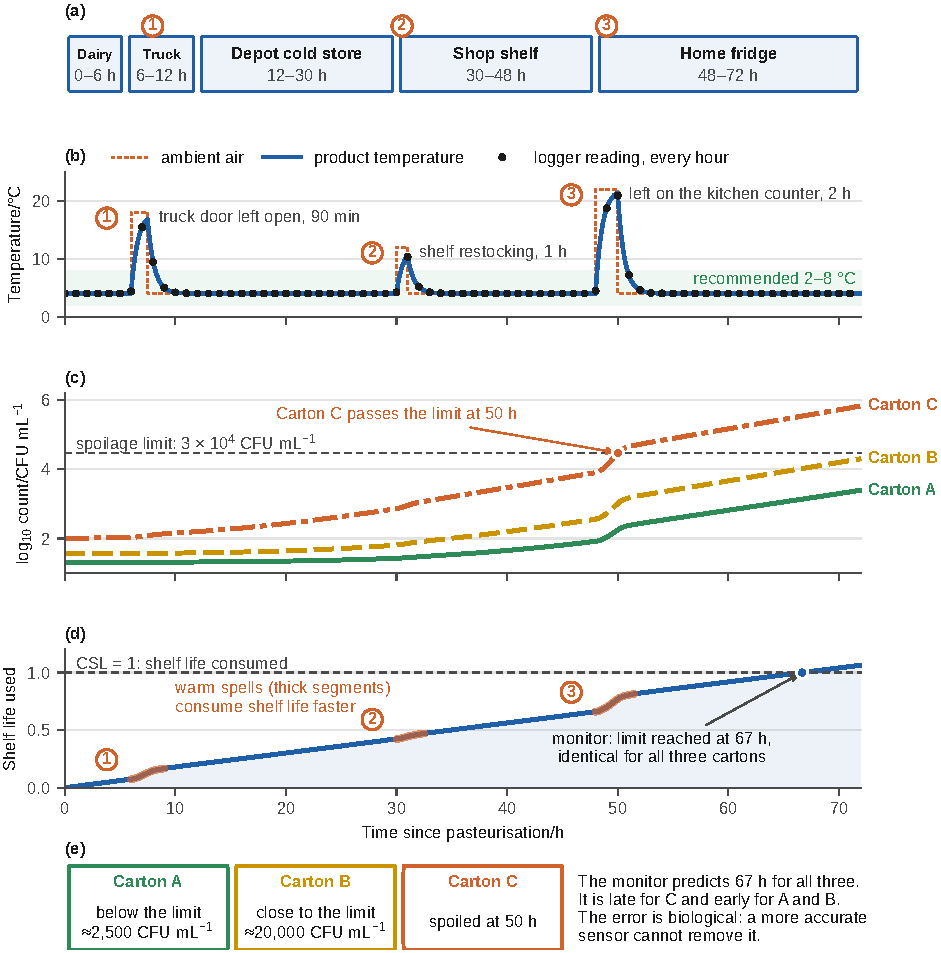
\includegraphics{story}
\caption{One delivery, three cartons. (a) Stages of a 72-h trip. (b) Ambient air and product temperature with three excursions, and the hourly logger readings. (c) Simulated counts in three cartons that share the same history but differ in starting load and lag. (d) Cumulative shelf life (CSL) computed by the monitor from the log; warm spells consume shelf life faster. (e) Outcome: one prediction for three cartons whose true fates differ}\label{fig:story}\end{figure*}

\subsection{An illustrative trip and the aim of the study}\label{sec:aim}
Figure~\ref{fig:story} shows the problem on a single trip. Three cartons travel together and therefore share one temperature history; they differ only in their starting load and the physiological state of their bacteria. A monitor that reads the log returns one answer for all three. It is late for one carton and early for the other two, and no improvement of the thermometer can change that, because the information it lacks is not in the temperature record. The aim of this study is to quantify that limit and to rank it against the losses a designer can control. Four research questions are addressed: (RQ1) how much ranking accuracy is lost to unobserved biology, to the sensor and to sampling; (RQ2) how much a better sensor or faster sampling recovers; (RQ3) how a growth-model score compares with simple rules on identical trips; and (RQ4) whether a probability is better calibrated than a single alarm.

\section{Models}\label{sec:models}
\subsection{Secondary model}
The square-root (Ratkowsky) law relates the maximum specific growth rate $\mu$ (h$^{-1}$, natural-log basis) to temperature below the optimum \cite{ratkowsky1982},
\begin{equation}\label{eq:sqrt}
\sqrt{\mu(T)} = b\,(T - T_{\min}), \qquad T > T_{\min}.
\end{equation}
Neumeyer fitted it to 68 growth curves of a fast-growing \textit{Pseudomonas} in broth and milk, giving $T_{\min}=-7.7$\degC{} and $b=0.030$\,h$^{-1/2}$\,K$^{-1}$ \cite{neumeyer1995}. Rates of \textit{P.~fluorescens} in UHT milk at 4, 15 and 29\degC{} \cite{lin2016} give $b=0.027$ and $T_{\min}=-9.0$\degC; the two sources agree within 15\,\% on generation time at 4\degC{} (5.6 and 6.4\,h). Equation~\eqref{eq:sqrt} implies $\mu(13)/\mu(4)=[(13-T_{\min})/(4-T_{\min})]^2=3.1$ for $T_{\min}=-7.7$\degC: one hour at 13\degC{} is worth about three hours at 4\degC.

\subsection{Reference model}
The Baranyi--Roberts model \cite{baranyi1993,baranyi1994}, which stands in for real milk, describes the log population $y=\ln N$ and a physiological state $q$:
\begin{align}
\frac{\dd y}{\dd t} &= \mu(T)\,\frac{q}{1+q}\left(1-\mathrm{e}^{\,y-y_{\max}}\right), \label{eq:bar}\\
\frac{\dd q}{\dd t} &= \mu(T)\,q, \qquad h_0=\ln\!\left(1+1/q_0\right).\label{eq:barq}
\end{align}
At constant temperature the lag is $\lambda=h_0/\mu$, so the product $\lambda\mu=h_0$ is constant for cells with the same history. The model handles changing temperature naturally, because $\mu$ is evaluated along the trace.

\subsection{Edge estimator}
The monitor itself uses a different primary model, so that the comparison is not circular. Let $\SL(T)$ be the time for a population at constant $T$ to reach a limit $N_L$ under the modified Gompertz curve \cite{zwietering1990},
\begin{equation}\label{eq:sl}
\SL(T) = \frac{h_0}{\mu(T)} + \frac{A}{\mu_{10}(T)\,\mathrm{e}}\left[1-\ln\!\left(-\ln\frac{L}{A}\right)\right],
\end{equation}
with $\mu_{10}=\mu/\ln 10$, $A=\log_{10}(N_{\max}/N_0)$ and $L=\log_{10}(N_L/N_0)$. A reading $T_i$ held over an interval $\Delta t_i$ consumes a fraction $\Delta t_i/\SL(T_i)$ of the shelf life, and the cumulative shelf life is
\begin{equation}\label{eq:csl}
\CSL = \sum_i \frac{\Delta t_i}{\SL(T_i)}, \qquad \text{limit reached when } \CSL\ge 1.
\end{equation}
Because every term of Eq.~\eqref{eq:sl} is proportional to $1/\mu$, $\SL(T)=K/\mu(T)$ with a constant $K$ that depends only on $h_0$, $N_0$, $N_L$ and $N_{\max}$, and therefore
\begin{equation}\label{eq:cslint}
\CSL=\frac{1}{K}\sum_i\mu(T_i)\,\Delta t_i\;\approx\;\frac{1}{K}\int_0^t\mu\big(T(s)\big)\dd s .
\end{equation}
The monitor thus integrates the growth rate along the log and compares the result with a fixed budget $K$. The temperature record determines the integral; the budget, which carries the biology, is not observed. Equation~\eqref{eq:csl} costs one table lookup and one addition per reading and runs on a microcontroller.

\section{Benchmark}\label{sec:bench}
\begin{figure*}[t]\centering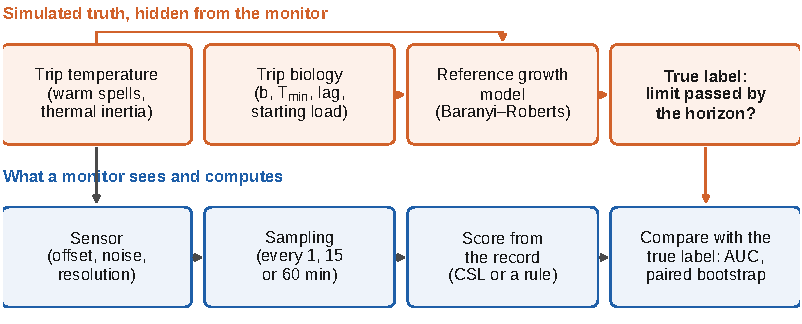
\includegraphics{design}
\caption{Design of the benchmark. Each simulated trip has a true temperature history and a true biology, which the reference model turns into a true label (top). The monitor sees only a sensed, sampled record and turns it into a score (bottom). Scores are judged against the true labels by AUC; removing information step by step gives the loss budget}\label{fig:design}\end{figure*}
Figure~\ref{fig:design} summarises the design: a simulated world supplies the truth, and a monitor that sees only a sensed, sampled record tries to recover it.

\subsection{Trips and labels}
Each trip has a product-temperature trace on a one-minute grid. The base temperature is drawn from 2.5--5\degC. Excursions arrive at a mean rate of one per 144\,h, peak at 12, 14.3, 17.5 or 30.7\degC{} (weights 0.30, 0.25, 0.30, 0.15) and last a lognormal time with median 60\,min, clipped to 10--480\,min. Product temperature follows ambient with a first-order time constant of 5--20\,min for a low-mass pouch and 1--4\,h for an insulated crate. A reference population grows along the trace by Eqs.~\eqref{eq:bar}--\eqref{eq:barq}, with $T_{\min}\sim\mathcal N(\bar T_{\min},\sigma_T^2)$, a lognormal multiplier on $b$ with coefficient of variation $cv\in\{0,0.10,0.25\}$, $h_0$ uniform over a measured range and a random starting load.

A trip is \emph{spoiled} if the reference population exceeds the limit within the label horizon, defined as the time the estimator takes to reach the limit at a constant 4\degC{} with nominal parameters, rounded up to a whole hour, as a printed shelf life would be. The horizon was fixed from label balance before any rule was compared. Prevalence is therefore constructed (about 0.5 for spoilage, \NumLisPrevMin--\NumLisPrevMax{} for \textit{Listeria}), and absolute predictive values must not be read as field rates.

\subsection{Sensors, sampling and scores}
Sensors add a per-trip offset, white noise and quantisation: a DS18B20 digital sensor (offset within $\pm0.5$\degC, noise 0.05\degC, step 0.0625\degC) \cite{ds18b20}, a PT1000 platinum resistance sensor read by a MAX31865 ($\pm0.15$\degC, 0.03\degC, 0.03125\degC) \cite{iec60751}, and an ideal sensor. Sampling intervals are 1, 15 and 60\,min, plus an adaptive rule that samples every minute while the temperature changes and every 15\,min otherwise. Five scores are computed from the measured record: $\CSL$; degree-hours above 4\degC; time above 5\degC; time above 8\degC; and maximum temperature. An \emph{oracle} $\CSL$ uses each trip's true parameters and noise-free temperature and sets the ceiling. In a structure-risk run, a quarter of the lag state is re-imposed whenever the product temperature departs from its two-hour running mean by more than 4\degC{} \cite{zwietering1994}; the estimator is not told about it.

\subsection{Parameter sets}
Table~\ref{tab:runs} lists the five runs. The baseline uses the Neumeyer parameters and a measured lag range. Because parameters from inoculated isolates need not describe natural flora, a fourth run uses parameters fitted to ComBase records of spoilage flora (\secref{sec:val}), and a fifth models \textit{Listeria monocytogenes} with labels of $+0.5$ and $+1$\,log$_{10}$ growth above the starting load (round-number labels, not regulatory limits). Each run has 12 settings (two limits, two products, three values of $cv$) of 4\,000 trips, so the benchmark contains 240\,000 trips, each read with every sensor, sampling rule and score.

\begin{table}[t]
\centering\footnotesize\caption{Benchmark runs. ``Assumed'' marks values without a source}\label{tab:runs}
\setlength{\tabcolsep}{4pt}
\begin{tabular}{@{}p{1.7cm}p{6.3cm}@{}}\toprule\rowcolor{dghead}
Run & Biology and labels\\\midrule
Baseline & $b=0.030$, $T_{\min}=-7.7$\degC{} \cite{neumeyer1995}; $\sigma_T=1.5$\,K (assumed); $h_0\in[2.5,5]$ \cite{lin2016}; $N_0$ 30--100\,CFU\,mL$^{-1}$ (assumed); limits $3\times10^4$ and $10^6$\,CFU\,mL$^{-1}$; horizons \NumBaseHzA{} and \NumBaseHzB\,h\\
Extra lag & as baseline, plus extra lag after shifts \cite{zwietering1994}\\
Low load & as baseline, $N_0$ 0.1--3\,CFU\,mL$^{-1}$ \cite{martin2021}; horizons \NumLowHzA{} and \NumLowHzB\,h\\
Milk flora & $b=\NumCbB$, $T_{\min}=\NumCbT$\degC{} (ComBase, $n=\NumCbNfit$), low load; horizons \NumCombHzA{} and \NumCombHzB\,h\\
\textit{Listeria} & $b=\NumLisB$, $T_{\min}=\NumLisT$\degC{} (ComBase, $n=\NumLisN$); $h_0\in[2,4.5]$, $\sigma_T=1.0$\,K, $N_0$ 0.06--0.18\,CFU\,mL$^{-1}$ (assumed); labels $+0.5$ and $+1$\,log; horizons \NumLisHzA{} and \NumLisHzB\,h\\\bottomrule
\end{tabular}
\end{table}

\subsection{Statistical analysis}\label{sec:stats}
The primary metric is the area under the ROC curve, $\AUC=\Pr(S_1>S_0)+\tfrac12\Pr(S_1=S_0)$, the probability that a randomly chosen spoiled trip scores higher than a randomly chosen unspoiled one \cite{hanley1982}. It depends on ranking, not on a threshold or on the constructed prevalence, and is estimated by the Mann--Whitney statistic \cite{mannwhitney1947}. Its standard error for $A=0.67$ and $n_1=n_0=2\,000$ is about 0.0085 by the Hanley--McNeil formula \cite{hanley1982}, which fixed the size of each setting: the biology gap is more than fifteen standard errors, while sensor and sampling effects are of the order of one and can be resolved only by paired comparison.

Two scores computed on the same trips are strongly correlated, so their difference $\hat D=\widehat{\AUC}_1-\widehat{\AUC}_2$ has variance $\mathrm{Var}(\widehat{\AUC}_1)+\mathrm{Var}(\widehat{\AUC}_2)-2\,\mathrm{Cov}(\widehat{\AUC}_1,\widehat{\AUC}_2)$, which is much smaller than the sum of the separate variances. Every trip is therefore read with every sensor, sampling rule and score (a common-random-numbers design), and intervals for differences come from a paired bootstrap of trips with $B=400$ resamples \cite{efron1993}, the resampling counterpart of the method of DeLong et al.\ \cite{delong1988}; single AUCs use $B=200$. No conclusion is drawn from a single setting: for each contrast the range over settings is reported, together with the number of settings whose 95\,\% interval excludes zero.

An uncertainty-aware variant draws $M=80$ parameter sets from a prior, computes $\CSL$ under each and reports the fraction that reach the limit as a probability. It is scored against a single alarm with nominal parameters by the Brier score \cite{brier1950} and by the expected calibration error over ten equal-width bins \cite{naeini2015}, $\mathrm{ECE}=\sum_m(|B_m|/n)\,|\bar y_{B_m}-\bar p_{B_m}|$.

\section{Validation against real data}\label{sec:val}
\subsection{A fluctuating-temperature experiment}
Lin et al.\ held UHT milk inoculated with \textit{P.~fluorescens} at 4\degC{} with two four-hour excursions to 29\degC, and report that the time to $10^6$\,CFU\,mL$^{-1}$ fell from about 90\,h to about 55\,h \cite{lin2016}. With parameters fitted only to their growth rates and their 4\degC{} lag, the reference model gives \NumLinConst\,h and \NumLinExc\,h, an error of $\NumLinErr$\,\% on the excursion case, which was not used for fitting. This is one experiment with one organism and an inoculated load far above real post-pasteurisation levels.

\subsection{Natural spoilage flora}
The \NumCbN{} ComBase records of aerobic spoilage bacteria in pasteurised milk span 2.7--14.9\degC{} \cite{combase}. One record (6.8\degC) lies far below its neighbours; without it the square-root law fits the remaining \NumCbNfit{} records with $b=\NumCbB$, $T_{\min}=\NumCbT$\degC{} and a residual standard deviation of \NumCbSd{} (natural-log units), and with it $b=\NumCbAllB$ and $T_{\min}=\NumCbAllT$\degC, so the conclusions do not depend on it. Parameters from inoculated isolates overpredict these records with a bias factor \cite{ross1996} of \NumCbBias{} that is nearly constant across temperature (Fig.~\ref{fig:cb}): the temperature \emph{shape} transfers from isolates to natural flora, the \emph{level} does not.

\begin{figure}[t]\centering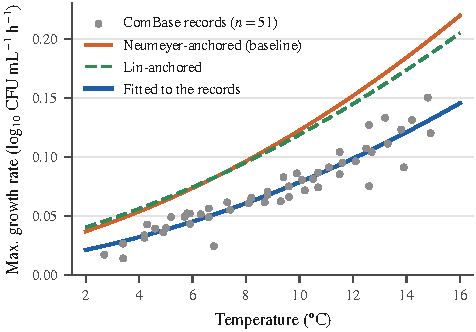
\includegraphics{combase}
\caption{Maximum growth rates of natural spoilage flora in pasteurised milk (points; ComBase \cite{combase}) with the Neumeyer-anchored model (dotted), the Lin-anchored model (dashed) and the square-root fit to the records (solid)}\label{fig:cb}\end{figure}

\subsection{\textit{Listeria monocytogenes}}
ComBase milk records with a stated rate for \textit{L.~monocytogenes} at 2--16\degC{} were split by condition: \NumLisN{} records without added factors were used for fitting and \NumLisHeld{} records with other stated conditions (sterilised or previously heated milk, added salts or acids) were held out. The fit gives $b=\NumLisB$ (95\,\% bootstrap interval \NumLisBLo--\NumLisBHi) and $T_{\min}=\NumLisT$\degC{} ($\NumLisTLo$ to $\NumLisTHi$\degC), a generation time of \NumLisGen\,h at 4\degC, and on the held-out records a bias factor of \NumLisBiasHeld{} and an accuracy factor of \NumLisAccHeld{} (\NumLisAccFit{} on the fitted records). Because $T_{\min}$ lies closer to refrigeration temperature, the rate at 13\degC{} is \NumLisRatio{} times that at 4\degC{} for \textit{Listeria}, against about 3.4 times for spoilage flora (Fig.~\ref{fig:lis}). The split is by condition rather than by study, so the test is weaker than a split by source.

\begin{figure*}[t]\centering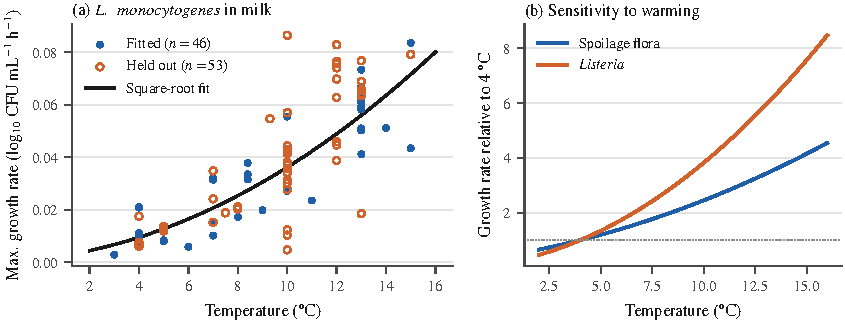
\includegraphics{lis}
\caption{\textit{Listeria monocytogenes} in milk. (a) Maximum growth rates used for fitting (filled) and held out by condition (open), with the square-root fit (ComBase \cite{combase}). (b) Growth rate relative to 4\degC{} for spoilage flora (solid) and \textit{Listeria} (dashed): a warm hour costs more for the pathogen}\label{fig:lis}\end{figure*}

\subsection{The compiled data}
ComBase returned about 480 records with milk as the food matrix, of which \DatNFull{} were compiled (Table~\ref{tab:dcomp}), together with the \DatNSp{} records of spoilage flora. All compiled records are released with the code.

\TabDataComp

\section{Results}\label{sec:results}
\begin{keyresults}
\begin{itemize}[leftmargin=1.1em]
\item Unobserved biology costs \NumBaseGapMin--\NumBaseGapMax{} AUC in the baseline run, an order of magnitude more than any sensor or sampling choice.
\item A PT1000 instead of a DS18B20 gains at most \NumBaseSensMax{} AUC; hourly sampling matches one-minute sampling in \NumBaseSampNull{} of 12 settings.
\item The kinetic score beats time above 5\degC{} and maximum temperature in every setting, but improves on degree-hours by at most \NumLagGainMax.
\item A Monte Carlo probability reaches ECE \NumBaseEceMMin--\NumBaseEceMMax; a single alarm \NumBaseEcePMin--\NumBaseEcePMax.
\end{itemize}
\end{keyresults}

\subsection{Loss budget (RQ1)}
An oracle that knows each trip's biology and temperature separates spoiled from unspoiled trips almost perfectly, by construction. The same $\CSL$ with nominal biology and an ideal sensor loses \NumBaseGapMin--\NumBaseGapMax{} AUC across the 12 baseline settings (Table~\ref{tab:budget}, Fig.~\ref{fig:budget}). The loss is large even when strains do not differ in growth rate ($cv=0$), because the minimum growth temperature, lag state and starting load still differ between trips. In terms of Eq.~\eqref{eq:cslint}, these quantities set the budget $K$ and the rate scale, which the temperature record does not contain; no sensor or sampling rate can recover them. Replacing the ideal sensor by a PT1000 or a DS18B20 sampled every 15 or 60\,min removes only a further 0.00--0.02.

\TabBudget

\begin{figure}[t]\centering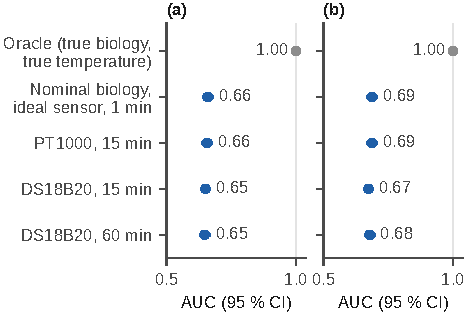
\includegraphics{budget}
\caption{Loss budget for (a) a low-mass pouch and (b) an insulated crate (limit $3\times10^4$\,CFU\,mL$^{-1}$, $cv=0.10$). Grey: oracle with true biology and temperature. Blue: the kinetic score as information is removed step by step. Bars: 95\,\% bootstrap intervals}\label{fig:budget}\end{figure}

\subsection{Sensors and sampling (RQ2)}
Replacing a DS18B20 with a PT1000 gains \NumBaseSensMin--\NumBaseSensMax{} AUC at 15-min sampling (Table~\ref{tab:contrasts}). A sensor offset of $\pm0.5$\degC{} shifts $\sqrt{\mu}$ by $b\times0.5$, about 4\,\% of its value at 4\degC, whereas the trip-to-trip spread of $T_{\min}$, $h_0$ and $N_0$ moves the shelf-life budget by tens of per cent; the ordering of the two losses follows directly. Sampling hourly instead of every minute shows no detectable difference in \NumBaseSampNull{} of 12 settings and at most about 0.01 where it does, and the adaptive rule is indistinguishable from fixed one-minute sampling. These results depend on the assumed excursion model (minimum duration 10\,min, median 60\,min) and would change if short, sharp excursions were common.

\TabContrasts

\subsection{Against simple rules (RQ3)}
On identical trips, the kinetic score beats time above 5\degC{} in \NumBaseFiveSig{} of 12 settings and maximum temperature in \NumBaseMaxSig{} (Table~\ref{tab:auc}). Against degree-hours above 4\degC, a rule that needs no growth model, the gain is positive with an interval excluding zero in \NumBaseGainSig{} of 12 settings but small: \NumBaseGainMin--\NumBaseGainMax{} AUC in the baseline run and up to \NumLagGainMax{} when extra lag is present. This is expected: near refrigeration temperature, Eq.~\eqref{eq:sqrt} is close to linear in $T$, so a degree-hour count is a first-order approximation of the integral in Eq.~\eqref{eq:cslint}. Most of the value of the kinetic score is therefore available from a degree-hour count; its advantage lies in the larger excursions, where the rate is strongly curved, and in its biological interpretation.

\TabAUC

\subsection{Robustness across parameter sets}
Figure~\ref{fig:runs} summarises the four effects across all five runs. The pattern holds whether the biology is anchored to inoculated isolates, includes extra lag, starts from a realistic low load, is fitted to natural flora or describes \textit{Listeria}: the biology gap is \NumLowGapMin--\NumLowGapMax{} (low load), \NumCombGapMin--\NumCombGapMax{} (milk flora) and \NumLisGapMin--\NumLisGapMax{} (\textit{Listeria}); the gain over degree-hours stays below \NumLagGainMax{} in every run; and the sensor gain stays small (\NumLisSensMin--\NumLisSensMax{} for \textit{Listeria}).

\begin{figure*}[t]\centering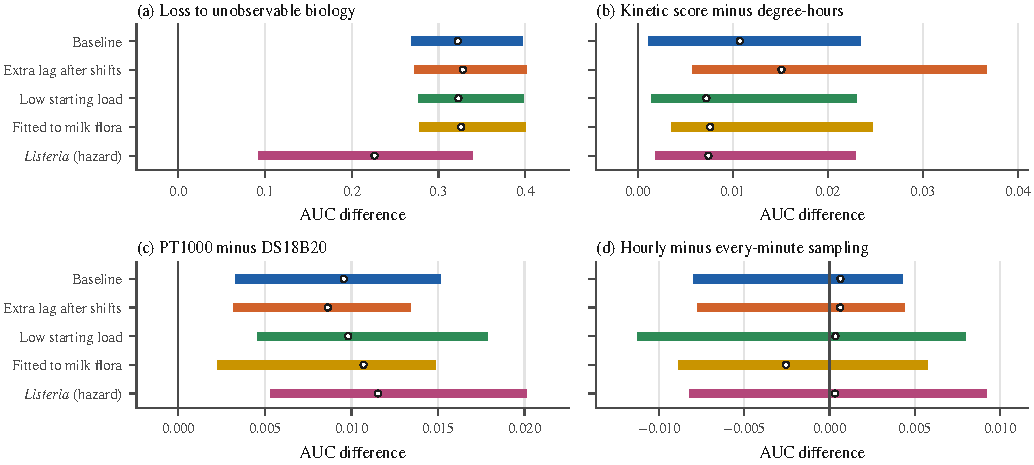
\includegraphics{runs}
\caption{Four effects across the five parameter sets, as AUC differences on identical trips: (a) loss to unobserved biology, (b) kinetic score over degree-hours, (c) PT1000 over DS18B20, (d) hourly over one-minute sampling. Bars span the 12 settings of each run; dots mark the median. Horizontal scales differ}\label{fig:runs}\end{figure*}

\subsection{Calibration (RQ4)}
A single alarm with nominal parameters is badly calibrated against the constructed labels (ECE \NumBaseEcePMin--\NumBaseEcePMax; Table~\ref{tab:cal}). A Monte Carlo probability with a prior that matches the truth reaches ECE \NumBaseEceMMin--\NumBaseEceMMax, and one with an overconfident prior on the growth rate \NumBaseEceOMin--\NumBaseEceOMax. Absolute values reflect the constructed prevalence; the ordering of the three variants is the finding. The \textit{Listeria} run requires a caveat. With the $+1$\,log label the probability reaches ECE \NumLisEceBMMin--\NumLisEceBMMax{} against \NumLisEceBPMin--\NumLisEceBPMax{} for the alarm. With the half-log label the limit falls inside the lag-to-growth transition, where the Gompertz estimator approximates the reference poorly; even the oracle reaches only \NumLisOrcAMin--\NumLisOrcAMax{} AUC there, and the probability, although still better than the alarm (ECE \NumLisEceAMMin--\NumLisEceAMMax{} against \NumLisEceAPMin--\NumLisEceAPMax), is poorly calibrated in absolute terms. The choice of label interacts with the structure of the estimator.

\TabCal

\section{Monitor architecture}\label{sec:toolkit}
Figure~\ref{fig:system} shows how the estimator runs on a logger. A probe reading is taken on an adaptive schedule, the shelf-life rate $1/\SL(T)$ is read from a stored table, Eq.~\eqref{eq:csl} is updated, and the same sum is carried for 80 sampled biological parameter sets to produce a probability. Parameter fitting is done once, offline. A browser demonstrator runs the same kernel (\url{https://copyninja07-07.github.io/dairyguard/}); a parity test ensures that it reproduces the Python implementation. A hardware logger is future work.

\begin{figure*}[t]\centering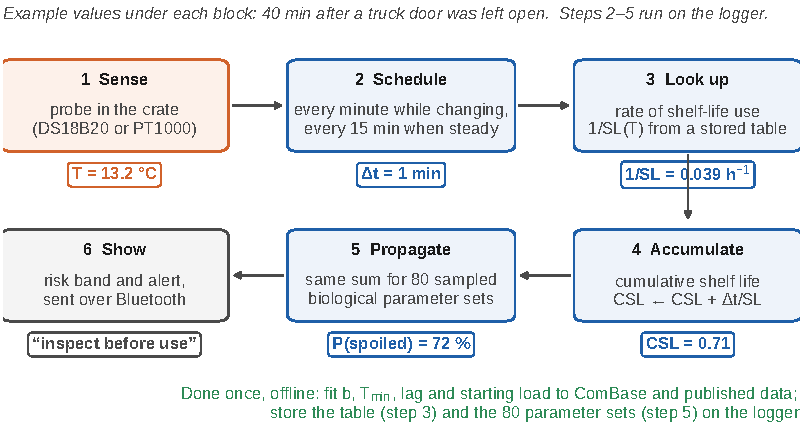
\includegraphics{system}
\caption{Processing on the logger, with example values 40\,min after a truck door was left open. Steps 2--5 run on the device; parameter fitting and the shelf-life table are prepared offline}\label{fig:system}\end{figure*}

\section{Discussion}\label{sec:disc}
\subsection{Where effort belongs}
In every run, what the thermometer cannot observe costs about an order of magnitude more accuracy than any choice of sensor or sampling interval. Equation~\eqref{eq:cslint} explains why: a log measures the integral of the growth rate well, but the budget against which the integral is compared varies from carton to carton. A more accurate thermometer is therefore a poor way to improve a spoilage estimate, and a low-cost digital probe sampled every 15--60\,min loses little under the assumptions made here. Effort is better spent on the biology: measuring the starting load or a proxy of handling history, learning the lag and strain spread of the product at hand, and reporting a probability instead of a verdict.

\subsection{Consistency with prior findings}
Sensitivity analyses rank temperature first \cite{lau2022,buehler2018,qian2023,giannakourou2020}; this study finds that biology dominates. The two results answer different questions. When temperature is drawn from a distribution, it drives the spread of outcomes; once it is measured, the residual uncertainty is biological. The small gain of the kinetic score over degree-hours agrees with the long practical use of degree-hour and time--temperature integrators \cite{taoukis1989,kim2020}.

\subsection{Hazard and spoilage}
For spoilage flora a warm hour is costly but the baseline rate is high; for \textit{Listeria}, growth at 4\degC{} is slow (generation time \NumLisGen\,h) but rises about \NumLisRatio-fold by 13\degC. The same benchmark and the same design conclusions hold for both. This paper does not estimate illness risk, which depends on dose, virulence, host and the contamination event, none of which are modelled.

\subsection{Limitations}
(i)~The reference and the estimator both reduce the temperature history to an integral of the growth rate, so the benchmark measures how much accuracy is lost to the listed sources, not whether a kinetic score models growth better; the structure-risk run relaxes one structural assumption only. (ii)~Strain spread, starting load, excursion statistics and the \textit{Listeria} lag are assumed. (iii)~Labels are constructed, with prevalence near 0.5 for spoilage and \NumLisPrevMin--\NumLisPrevMax{} for \textit{Listeria}. (iv)~ComBase records come from heterogeneous studies and report maximum rates, not curves, so lag and responses to shifts are untested on them. (v)~A single experiment validates fluctuating temperature, and no new plate counts were made. (vi)~Neither organism class represents spore-formers, which account for a large share of spoilage \cite{martin2021}.

\section{Conclusions}\label{sec:concl}
A temperature log can say much about how much growth the milk \emph{could} have had, and little about how much it \emph{did}. In an open benchmark of 240\,000 trips anchored to published and ComBase data, unobserved biology costs \NumBaseGapMin--\NumBaseGapMax{} AUC; a degree-hour count comes within \NumLagGainMax{} of a growth model; sensor quality and sampling interval matter little; and a Monte Carlo probability is far better calibrated than an alarm. Direct measurement of biology and of growth under fluctuating temperature, with new plate counts, is the next step. The kinetic basis of these findings, in particular why simple temperature integrators come so close to a growth model, is the subject of an extended study in preparation.

\section*{Acknowledgements}
The author thanks Dr.\ Neeraj Tripathi (School of Electronics and Communication Engineering, Shri Mata Vaishno Devi University) for guidance, and the ComBase consortium and the laboratories whose published growth records made this study possible.

\section*{Data and code availability}
Code, 14 automated tests, the parameter file with the source of every value, all simulation results and the compiled ComBase milk records are available at \url{https://github.com/CopyNinja07-07/dairyguard}; \texttt{make all} reproduces every table and figure from fixed random seeds, and every number in this paper is written from the result files by a script. Numerical work uses NumPy, SciPy and Matplotlib \cite{harris2020,virtanen2020,hunter2007}. Parts of the simulation code were developed with an AI coding assistant; all of it is covered by the automated tests and was checked by the author. ComBase records remain subject to the ComBase terms of use.

{\scriptsize\linespread{0.94}\selectfont
\makeatletter\renewcommand\@biblabel[1]{#1.}\makeatother
\begin{thebibliography}{99}
\setlength{\itemsep}{0pt}
\bibitem{perez2013} Pérez-Rodríguez F, Valero A. Predictive microbiology in foods. New York: Springer; 2013. \url{https://doi.org/10.1007/978-1-4614-5520-2}
\bibitem{tarlak2023} Tarlak F. The use of predictive microbiology for the prediction of the shelf life of food products. Foods. 2023;12:4461. \url{https://doi.org/10.3390/foods12244461}
\bibitem{stavropoulou2019} Stavropoulou E, Bezirtzoglou E. Predictive modeling of microbial behavior in food. Foods. 2019;8:654. \url{https://doi.org/10.3390/foods8120654}
\bibitem{vyazovkin2011} Vyazovkin S, Burnham AK, Criado JM, Pérez-Maqueda LA, Popescu C, Sbirrazzuoli N. ICTAC Kinetics Committee recommendations for performing kinetic computations on thermal analysis data. Thermochim Acta. 2011;520:1--19. \url{https://doi.org/10.1016/j.tca.2011.03.034}
\bibitem{vyazovkin2015} Vyazovkin S. Isoconversional kinetics of thermally stimulated processes. Cham: Springer; 2015. \url{https://doi.org/10.1007/978-3-319-14175-6}
\bibitem{koga2023} Koga N, Vyazovkin S, Burnham AK, et al. ICTAC Kinetics Committee recommendations for analysis of thermal decomposition kinetics. Thermochim Acta. 2023;719:179384. \url{https://doi.org/10.1016/j.tca.2022.179384}
\bibitem{ozawa1965} Ozawa T. A new method of analyzing thermogravimetric data. Bull Chem Soc Jpn. 1965;38:1881--6. \url{https://doi.org/10.1246/bcsj.38.1881}
\bibitem{ozawa1986} Ozawa T. Non-isothermal kinetics and generalized time. Thermochim Acta. 1986;100:109--18. \url{https://doi.org/10.1016/0040-6031(86)87053-8}
\bibitem{koga2013} Koga N. Ozawa's kinetic method for analyzing thermoanalytical curves: history and theoretical fundamentals. J Therm Anal Calorim. 2013;113:1527--41. \url{https://doi.org/10.1007/s10973-012-2882-5}
\bibitem{malek2013} Málek J, Koga N, Pérez-Maqueda LA, Criado JM. The Ozawa's generalized time concept and YZ-master plots as a convenient tool for kinetic analysis of complex processes. J Therm Anal Calorim. 2013;113:1437--46. \url{https://doi.org/10.1007/s10973-013-2939-0}
\bibitem{schiraldi2019} Schiraldi A, Fessas D. Calorimetry and thermal analysis in food science. J Therm Anal Calorim. 2019;138:2721--32. \url{https://doi.org/10.1007/s10973-019-08166-z}
\bibitem{fessas2017} Fessas D, Schiraldi A. Isothermal calorimetry and microbial growth: beyond modeling. J Therm Anal Calorim. 2017;130:567--72. \url{https://doi.org/10.1007/s10973-017-6515-x}
\bibitem{wadso2011} Wadsö L, Salamanca Y, Johansson S. Biological applications of a new isothermal calorimeter that simultaneously measures at four temperatures. J Therm Anal Calorim. 2011;104:119--26. \url{https://doi.org/10.1007/s10973-010-1140-y}
\bibitem{haman2019} Haman N, Signorelli M, Duce C, Franzetti L, Fessas D. Isothermal calorimetry protocols to monitor the shelf life and aftermarket follow-up of fresh cut vegetables. J Therm Anal Calorim. 2019;137:1673--80. \url{https://doi.org/10.1007/s10973-019-08064-4}
\bibitem{fricke2020} Fricke C, Harms H, Maskow T. How to speed up the detection of aerobic microbial contaminations by using isothermal microcalorimetry. J Therm Anal Calorim. 2020;142:1933--49. \url{https://doi.org/10.1007/s10973-020-09986-0}
\bibitem{martin2021} Martin NH, Torres-Frenzel P, Wiedmann M. Invited review: controlling dairy product spoilage to reduce food loss and waste. J Dairy Sci. 2021;104:1251--61. \url{https://doi.org/10.3168/jds.2020-19130}
\bibitem{ranieri2009} Ranieri ML, Boor KJ. Short communication: bacterial ecology of high-temperature, short-time pasteurized milk processed in the United States. J Dairy Sci. 2009;92:4833--40. \url{https://doi.org/10.3168/jds.2009-2181}
\bibitem{who2015} World Health Organization. WHO's first ever global estimates of foodborne diseases find children under 5 account for almost one third of deaths. News release, 3 December 2015. \url{https://www.who.int/news/item/03-12-2015-who-s-first-ever-global-estimates-of-foodborne-diseases-find-children-under-5-account-for-almost-one-third-of-deaths}
\bibitem{fssai2024} Food Safety and Standards Authority of India. Appendix B: microbiological requirements, version 2 (4 November 2024), Tables 2A and 2B. \url{https://fssai.gov.in/upload/uploadfiles/files/Appendix%20B(1).pdf}
\bibitem{badiamelis2018} Badia-Melis R, Mc Carthy U, Ruiz-Garcia L, Garcia-Hierro J, Robla Villalba JI. New trends in cold chain monitoring applications -- a review. Food Control. 2018;86:170--82. \url{https://doi.org/10.1016/j.foodcont.2017.11.022}
\bibitem{mercier2017} Mercier S, Villeneuve S, Mondor M, Uysal I. Time--temperature management along the food cold chain: a review of recent developments. Compr Rev Food Sci Food Saf. 2017;16:647--67. \url{https://doi.org/10.1111/1541-4337.12269}
\bibitem{jedermann2014} Jedermann R, Nicometo M, Uysal I, et al. Reducing food losses by intelligent food logistics. Philos Trans R Soc A. 2014;372:20130302. \url{https://doi.org/10.1098/rsta.2013.0302}
\bibitem{koutsoumanis2005} Koutsoumanis K, Taoukis PS, Nychas G-JE. Development of a Safety Monitoring and Assurance System for chilled food products. Int J Food Microbiol. 2005;100:253--60. \url{https://doi.org/10.1016/j.ijfoodmicro.2004.10.024}
\bibitem{goransson2018} Göransson M, Nilsson F, Jevinger Å. Temperature performance and food shelf-life accuracy in cold food supply chains: insights from multiple field studies. Food Control. 2018;86:332--41. \url{https://www.sciencedirect.com/science/article/pii/S0956713517305145}
\bibitem{kim2020} Kim J, Santos CA, Kim B-S, Kim J, Koo J. Estimation of real-time remaining shelf life using mean kinetic temperature. LWT. 2020;134:109968. \url{https://doi.org/10.1016/j.lwt.2020.109968}
\bibitem{lima2026} Lima L, Pereira AI, Pintado M, Carocho M. Fresh dairy quality in the era of smart food systems: deterioration pathways, analytical technologies, and predictive modeling. Foods. 2026;15:3439. \url{https://doi.org/10.3390/foods15193439}
\bibitem{corradini2005} Corradini MG, Peleg M. Estimating non-isothermal bacterial growth in foods from isothermal experimental data. J Appl Microbiol. 2005;99:187--200. \url{https://doi.org/10.1111/j.1365-2672.2005.02570.x}
\bibitem{gompertz1825} Gompertz B. On the nature of the function expressive of the law of human mortality, and on a new mode of determining the value of life contingencies. Philos Trans R Soc Lond. 1825;115:513--83. \url{https://doi.org/10.1098/rstl.1825.0026}
\bibitem{zwietering1990} Zwietering MH, Jongenburger I, Rombouts FM, van 't Riet K. Modeling of the bacterial growth curve. Appl Environ Microbiol. 1990;56:1875--81. \url{https://doi.org/10.1128/aem.56.6.1875-1881.1990}
\bibitem{baranyi1993} Baranyi J, Roberts TA, McClure P. A non-autonomous differential equation to model bacterial growth. Food Microbiol. 1993;10:43--59. \url{https://doi.org/10.1006/fmic.1993.1005}
\bibitem{baranyi1994} Baranyi J, Roberts TA. A dynamic approach to predicting bacterial growth in food. Int J Food Microbiol. 1994;23:277--94. \url{https://doi.org/10.1016/0168-1605(94)90157-0}
\bibitem{ratkowsky1982} Ratkowsky DA, Olley J, McMeekin TA, Ball A. Relationship between temperature and growth rate of bacterial cultures. J Bacteriol. 1982;149:1--5. \url{https://doi.org/10.1128/jb.149.1.1-5.1982}
\bibitem{rosso1993} Rosso L, Lobry JR, Flandrois JP. An unexpected correlation between cardinal temperatures of microbial growth highlighted by a new model. J Theor Biol. 1993;162:447--63. \url{https://doi.org/10.1006/jtbi.1993.1099}
\bibitem{baranyi2004} Baranyi J, Tamplin ML. ComBase: a common database on microbial responses to food environments. J Food Prot. 2004;67:1967--71. \url{https://doi.org/10.4315/0362-028X-67.9.1967}
\bibitem{combase} ComBase. Database of microbial responses to food environments: growth records with milk as the food matrix. Accessed 19 Oct 2026. \url{https://www.combase.cc}
\bibitem{neumeyer1995} Neumeyer K. Modelling pseudomonad growth in milk and milk-based products. Research Master thesis. Hobart: University of Tasmania; 1995. \url{https://eprints.utas.edu.au/21013/}
\bibitem{neumeyer1997a} Neumeyer K, Ross T, McMeekin TA. Development of a predictive model to describe the effects of temperature and water activity on the growth of spoilage pseudomonads. Int J Food Microbiol. 1997;38:45--54. \url{https://doi.org/10.1016/S0168-1605(97)00089-5}
\bibitem{lin2016} Lin H, Shavezipur M, Yousef A, Maleky F. Prediction of growth of \textit{Pseudomonas fluorescens} in milk during storage under fluctuating temperature. J Dairy Sci. 2016;99:1822--30. \url{https://doi.org/10.3168/jds.2015-10179}
\bibitem{zwietering1994} Zwietering MH, de Wit JC, Cuppers HGAM, van 't Riet K. Modeling of bacterial growth with shifts in temperature. Appl Environ Microbiol. 1994;60:204--13. \url{https://doi.org/10.1128/aem.60.1.204-213.1994}
\bibitem{riva2001} Riva M, Fessas D, Schiraldi A. Isothermal calorimetry approach to evaluate shelf life of foods. Thermochim Acta. 2001;370:73--81. \url{https://doi.org/10.1016/S0040-6031(00)00782-6}
\bibitem{juneja2011} Juneja VK, Huang L, Yan X. Thermal inactivation of foodborne pathogens and the USDA pathogen modeling program. J Therm Anal Calorim. 2011;106:191--8. \url{https://doi.org/10.1007/s10973-011-1453-5}
\bibitem{nauta2000} Nauta MJ. Separation of uncertainty and variability in quantitative microbial risk assessment models. Int J Food Microbiol. 2000;57:9--18. \url{https://doi.org/10.1016/S0168-1605(00)00225-7}
\bibitem{lau2022} Lau S, Trmčić A, Martin NH, Wiedmann M, Murphy SI. Development of a Monte Carlo simulation model to predict pasteurized fluid milk spoilage due to post-pasteurization contamination with gram-negative bacteria. J Dairy Sci. 2022;105:1978--98. \url{https://doi.org/10.3168/jds.2021-21316}
\bibitem{buehler2018} Buehler AJ, Martin NH, Boor KJ, Wiedmann M. Psychrotolerant spore-former growth characterization for the development of a dairy spoilage predictive model. J Dairy Sci. 2018;101:6964--81. \url{https://doi.org/10.3168/jds.2018-14501}
\bibitem{qian2023} Qian C, Murphy SI, Lott TT, Martin NH, Wiedmann M. Development and deployment of a supply-chain digital tool to predict fluid-milk spoilage due to psychrotolerant sporeformers. J Dairy Sci. 2023;106:8414--33. \url{https://doi.org/10.3168/jds.2023-23673}
\bibitem{giannakourou2020} Giannakourou MC, Taoukis PS. Holistic approach to the uncertainty in shelf life prediction of frozen foods at dynamic cold chain conditions. Foods. 2020;9:714. \url{https://doi.org/10.3390/foods9060714}
\bibitem{taoukis1989} Taoukis PS, Labuza TP. Applicability of time-temperature indicators as shelf life monitors of food products. J Food Sci. 1989;54:783--8. \url{https://doi.org/10.1111/j.1365-2621.1989.tb07882.x}
\bibitem{fu1991} Fu B, Taoukis PS, Labuza TP. Predictive microbiology for monitoring spoilage of dairy products with time-temperature integrators. J Food Sci. 1991;56:1209--15. \url{https://doi.org/10.1111/j.1365-2621.1991.tb04736.x}
\bibitem{koutsoumanis2001} Koutsoumanis K. Predictive modeling of the shelf life of fish under nonisothermal conditions. Appl Environ Microbiol. 2001;67:1821--9. \url{https://doi.org/10.1128/AEM.67.4.1821-1829.2001}
\bibitem{zou2023} Zou Y, Wu J, Wang X, Morales K, Liu G, Manzardo A. An improved artificial neural network using multi-source data to estimate food temperature during multi-temperature delivery. J Food Eng. 2023;351:111518. \url{https://doi.org/10.1016/j.jfoodeng.2023.111518}
\bibitem{muller2026} Müller WA, Kronbauer M, Ferreira SB, da Silva SB. Computational assessment of temperature failures in the cold supply chain: implications for beef shelf life. Food Control. 2026;187:112100. \url{https://doi.org/10.1016/j.foodcont.2026.112100}
\bibitem{ndraha2018} Ndraha N, Hsiao H-I, Vlajic J, Yang M-F, Lin H-TV. Time-temperature abuse in the food cold chain: review of issues, challenges, and recommendations. Food Control. 2018;89:12--21. \url{https://doi.org/10.1016/j.foodcont.2018.01.027}
\bibitem{sofat2026} Sofat A, Sodhi B. Beyond thresholds: a quality-aware decision intelligence framework for cold chain IoT systems. arXiv preprint arXiv:2608.15082. 2026. \url{https://arxiv.org/abs/2608.15082}
\bibitem{singh2026} Singh SP. How much can a temperature log tell us about spoiling milk? A loss-budget benchmark for cold-chain monitoring. Preprint; 2026. Version 1. \url{https://copyninja07-07.github.io/dairyguard/DairyGuard_Preprint_v1.pdf}
\bibitem{efron1993} Efron B, Tibshirani RJ. An introduction to the bootstrap. New York: Chapman \& Hall; 1993. \url{https://doi.org/10.1201/9780429246593}
\bibitem{arrhenius1889} Arrhenius S. Über die Reaktionsgeschwindigkeit bei der Inversion von Rohrzucker durch Säuren. Z Phys Chem. 1889;4:226--48. \url{https://doi.org/10.1515/zpch-1889-0416}
\bibitem{ozawa1970} Ozawa T. Kinetic analysis of derivative curves in thermal analysis. J Therm Anal. 1970;2:301--24. \url{https://doi.org/10.1007/BF01911411}
\bibitem{ds18b20} Analog Devices (Maxim Integrated). DS18B20 programmable resolution 1-Wire digital thermometer. Product page and datasheet. \url{https://www.analog.com/en/DS18B20}
\bibitem{iec60751} International Electrotechnical Commission. IEC 60751:2022 Industrial platinum resistance thermometers and platinum temperature sensors. Geneva: IEC; 2022. \url{https://webstore.iec.ch/en/publication/63753}
\bibitem{hanley1982} Hanley JA, McNeil BJ. The meaning and use of the area under a receiver operating characteristic (ROC) curve. Radiology. 1982;143:29--36. \url{https://doi.org/10.1148/radiology.143.1.7063747}
\bibitem{mannwhitney1947} Mann HB, Whitney DR. On a test of whether one of two random variables is stochastically larger than the other. Ann Math Stat. 1947;18:50--60. \url{https://doi.org/10.1214/aoms/1177730491}
\bibitem{delong1988} DeLong ER, DeLong DM, Clarke-Pearson DL. Comparing the areas under two or more correlated receiver operating characteristic curves: a nonparametric approach. Biometrics. 1988;44:837--45. \url{https://doi.org/10.2307/2531595}
\bibitem{brier1950} Brier GW. Verification of forecasts expressed in terms of probability. Mon Weather Rev. 1950;78:1--3. \url{https://doi.org/10.1175/1520-0493(1950)078<0001:VOFEIT>2.0.CO;2}
\bibitem{naeini2015} Naeini MP, Cooper GF, Hauskrecht M. Obtaining well calibrated probabilities using Bayesian binning. Proc AAAI Conf Artif Intell. 2015;29:2901--7. \url{https://doi.org/10.1609/aaai.v29i1.9602}
\bibitem{akaike1974} Akaike H. A new look at the statistical model identification. IEEE Trans Autom Control. 1974;19:716--23. \url{https://doi.org/10.1109/TAC.1974.1100705}
\bibitem{hurvich1989} Hurvich CM, Tsai C-L. Regression and time series model selection in small samples. Biometrika. 1989;76:297--307. \url{https://doi.org/10.1093/biomet/76.2.297}
\bibitem{ross1996} Ross T. Indices for performance evaluation of predictive models in food microbiology. J Appl Bacteriol. 1996;81:501--8. \url{https://doi.org/10.1111/j.1365-2672.1996.tb03539.x}
\bibitem{harris2020} Harris CR, Millman KJ, van der Walt SJ, et al. Array programming with NumPy. Nature. 2020;585:357--62. \url{https://doi.org/10.1038/s41586-020-2649-2}
\bibitem{virtanen2020} Virtanen P, Gommers R, Oliphant TE, et al. SciPy 1.0: fundamental algorithms for scientific computing in Python. Nat Methods. 2020;17:261--72. \url{https://doi.org/10.1038/s41592-019-0686-2}
\bibitem{hunter2007} Hunter JD. Matplotlib: a 2D graphics environment. Comput Sci Eng. 2007;9:90--5. \url{https://doi.org/10.1109/MCSE.2007.55}
\end{thebibliography}
}

\end{document}
